\documentclass[conference, a4paper]{IEEEtran}
\IEEEoverridecommandlockouts
% The preceding line is only needed to identify funding in the first footnote. If that is unneeded, please comment it out.
\usepackage[utf8]{inputenc}
\usepackage{cite}
\usepackage{amsmath,amssymb,amsfonts}
\usepackage{algorithmic}
\usepackage{listings}
\usepackage{algorithm}
\usepackage{graphicx}
\usepackage{textcomp}
\usepackage{xcolor}
\def\BibTeX{{\rm B\kern-.05em{\sc i\kern-.025em b}\kern-.08em
    T\kern-.1667em\lower.7ex\hbox{E}\kern-.125emX}}
\begin{document}
\lstset{
%  basicstyle=\ttfamily,
%  columns=fullflexible,
%  frame=single,
  breaklines=true,
  postbreak=\mbox{\textcolor{red}{$\hookrightarrow$}\space},
}

\title{Real-time processing of cybersecurity system data for attacker profiling\\
%{\footnotesize \textsuperscript{*}Note: Sub-titles are not captured in Xplore and should not be used}
\thanks{This research is funded by the VVGS projects under contract No. VVGS-PF-2019-1062, VEGA project under contract No. VEGA/A-1/0056/18, and Slovak Research and development agency (SRDA) project under contract No. APVV-17-0561.}
}

\author{\IEEEauthorblockN{1\textsuperscript{st} Patrik Pekarčík}
\IEEEauthorblockA{\textit{Computer science institute} \\
\textit{Pavol Jozef Safarik University}\\
Košice, Slovakia \\
patrik.pekarcik@student.upjs.sk}
\and
\IEEEauthorblockN{2\textsuperscript{nd} Tomáš Kekeňák}
\IEEEauthorblockA{\textit{Computer science institute} \\
\textit{Pavol Jozef Safarik University}\\
Košice, Slovakia \\
tomas.kekenak@student.upjs.sk}
\and
\IEEEauthorblockN{3\textsuperscript{rd} Pavol Sokol}
\IEEEauthorblockA{\textit{Computer science institute} \\
\textit{Pavol Jozef Safarik University}\\
Košice, Slovakia \\
pavol.sokol@upjs.sk}
\and
\IEEEauthorblockN{4\textsuperscript{th} Terézia Mézešová}
\IEEEauthorblockA{\textit{Computer science institute} \\
\textit{Pavol Jozef Safarik University}\\
Košice, Slovakia \\
terezia.mezesova@upjs.sk}
}

\maketitle

\begin{abstract}
Usage of cybersecurity tools entails an enormous amount of data that brings the possibility of different approaches to the processing of cybersecurity data. This paper discusses the profiling of attackers, which, in practice, can help in managing cybersecurity events. The main goal of the research is to perform attackers' profiling as close as possible to real-time processing. The paper outlines the basic idea of real-time attacker profiling. We use stream processing. Within the system, we profile attackers into seven profiles or mark them as outliers if they do not fall into any of the known profiles. The paper also deals with the dynamic profiling model update and the difference of the calculated model using the original non-real-time model.
\end{abstract}

\begin{IEEEkeywords}
attacker profiling, real-time stream processing, classification, cybersecurity data
\end{IEEEkeywords}

\section{Introduction}
As the number of heterogeneous devices in computer networks increases, the number of security incidents that security analysts must address is also increasing. Among the standard devices we encounter in the current computer networks, we can include mobile phones, Internet of Things (IoT) devices, such as smart coffee machines, valves, locks. Host-based defence solutions, such as antivirus, are impractical for these devices due to their high consumption of resources. For this reason, network security specialises in monitoring network traffic, tracking application logs from specific devices, network devices or network services. We can name these solutions as passive because they do not limit the work of the devices. Since we are dealing with monitoring network traffic, we have to think about a large amount of data and look for a solution which will be very responsive to changes in network security data. 

All the mentioned data is flowing continuously to the central security unit. In this type of big data application, it is not necessary to process entire data at once. Most of big data applications are just streaming current data to processing units \cite{mizell2017introduction}. This type of processing is called Stream Processing. It allows applications to efficiently exploit a limited form of parallel processing, without explicitly managing allocation, synchronisation or communication among these units \cite{cugola2012processing}.

This paper aims to design and implement a real-time classification of a threat. Threat profiling consists of extracting behaviour characteristics of detected threats and clustering them into distinct groups called profiles and subsequently classifying any incoming threats into the predefined profiles. To achieve this aim, we build on the research of attacker profiling in \cite{bajtovs2018network}. Mentioned research is comparing several methods for creating clusters of a threat. They found that partitioning around medoids (PAM) clustering method will act with good results. Also, they reasonably discuss the number of searching clusters and seven clusters acted with cleaner results - internal measures and stability measure in combination witch external facts indicated seven as an appropriate number of clusters.
The problem identifies in the research is that the potential attack is revealed with a considerable time delay. A status alert that includes two-week data is not as relevant as an alert about current activity. We extend the profile of attackers used in this way in order to classify attackers in real-time using a streaming approach. The principle of current processing is data stream processing and verification of fulfilment of conditions of set computational models. This type of processing performs the data calculations within a short time after receiving the data. Usually, it takes from milliseconds to minutes. 
Profiles adapting to the new incoming threats in real-time is an active research area proposed in the reviewed literature.
Based on the above, we state the following research sub-goals:
    \begin{enumerate}
        \item design a model for real-time profiling, and
        \item design and implement a system for real-time profiling.
    \end{enumerate}

This paper is organised into five sections. Section II focuses on~the~review of the published papers on profiling and related topics. Section III outlines the dataset. Section IV focuses on the design and implementation of a system for real-time profiling. In Section V, we outline the model of real-time profiling, including aggregation, classification, model actualisation and results. The~last section contains conclusions and~suggestions for~the~future research.

\section{State of art}

Usage of the k-means clustering method on network data was proposed in \cite{marchette1999statistical} to create various activity groups and thus identify any abnormal activity on the network.
Wang, Hu and Hu surveyed the approaches towards profiling the behaviour of network traffic of target hosts in \cite{wang2019survey}. They presented various techniques which differ in the kind of network data that is used to extract the profile defining features. They identified profiling based on multi-source information and lack of consensus on evaluation metrics as still open issues.
Network backbone traffic was profiled to detect anomalies in \cite{zang2019adaptive}. Over 40 attributes characterised the profiles. Ant colony optimisation algorithm was used to find the anomalies. Their experimental results showed an accuracy of 97.4\% and false positive rate of 0.9\%.
In \cite{xu2014behavior}, communication between hosts in a backbone network was modelled as a bipartite graph and clustering are performed based on the closeness of the nodes, defined by a clustering coefficient which can be applied both locally or globally. It is an adapted, simple spectral clustering algorithm. There were also described the practical benefits of exploring the behaviour of network end-hosts, such as detecting scanning activities, early phases of worms, distributed DoS attacks.
Hammerschmidt et al. proposed an approach in \cite{hammerschmidt2016efficient} towards learning and distinguishing among various profiles in network communication which requires a small number of attributes. Probabilistic deterministic finite automata were adapted and required less training data. The objective of the profiling module is to distinguish between legitimate and botnet traffic.
In \cite{berti2017profiling}, the authors presented a pipeline where they can identify and cluster together typical attack profiles, focusing on detection of distributed reflective DoS attacks. They identified 13 clusters. Various clustering algorithms were tested (k-means, self-organising maps, expectation maximisation, and others).
DBSCAN algorithm identified in \cite{jakalan2015profiling} 5 profiles of attack behaviour - scanning a single port, port scanning on a single host, server traffic behaviour, clients sending HTTP-like requests, P2P traffic.
In \cite{bakhshi2015user}, k-means clustering was used for Netflow records. Their results were 4 clusters, each characterised by nine attributes. 

The reviewed related works focus on the creation of the model in an offline mode, where all the learning data is available, and no new data is incoming. In their future works section, they mention that the next stage of the research is performing the techniques in real-time. We describe our approach to it in this paper.


\section{Dataset}
The source of data for our research is the alerts obtained from a Warden system \cite{kacha2015warden}. It is a system that supports sharing information about security events on individual computer networks connected to this system. Data is stored and shared in IDEA format (Intrusion Detection Extensible Alert) \cite{kacha2014idea}. IDEA format is a descriptive data model using a key-value JSON structure. The main detection sources of data that send IDEA alerts to the Warden system can include attack detection systems, honeypots, network flow probes, system log records. Alert in the IDEA format contains several mandatory attributes (format, ID, detect time, category) \cite{kacha2013idea} and many optional fields with multiple input support. The fields we follow most in this research are the category, network traffic source data (IP address, port, protocol), network traffic target data (IP, port, protocol), detection time, and interruption time. For this research, data were collected during four weeks (from 2018-01-12 to 2018-02-09) by the Warden system. We have split security data into four parts per each week. Collected data contain approximately 216 million records from various data sources mentioned above.

In Tab.~\ref{tab:dataset_categories} it is shown the specific attributes of each analysis weak, especially number of IP address, number of the Internet service providers, average of security incident category - recon scanning. 

\begin{table}[ht]
\centering
\caption{Information about weeks in dataset}
\label{tab:dataset_categories}
 \begin{tabular}{|c|c|c|c|c|c|} 
    \hline
    Week & No. IP & No. ISP & Avg of Cat. Recon-scanning  \\
    \hline
    \textbf{Week 1} & 546 359 & 16 004 & 9.33 \\
    \textbf{Week 2} & 528 982 & 15 832 & 10.18 \\
    \textbf{Week 3} & 497 512 & 15 915 & 10.92 \\
    \textbf{Week 4} & 520 800 & 15 887 & 11.00 \\
    \hline
 \end{tabular}
\end{table}


\section{Design and implementation of a system for real-time profiling}

We now present the input data and the way of their current aggregation and subsequent classification. We describe the processing of security data in individual processing steps. We have verified this approach using the Python scripts with the usage of PostgreSQL memory database. The following diagram (Fig.~\ref{fig1}) shows how we designed the profiling of attackers by using security data stream processing. It is a module to simplify the definition of individual processing steps and communication between them. The schema contains separate processing steps to receive events continually. The events are then processed according to the current processing step and responded by sending the processed data to the next processing step. Some processing steps are illustrated with pseudocode for a better understanding of processing complexity at them. 

\begin{figure}[htbp]
\centerline{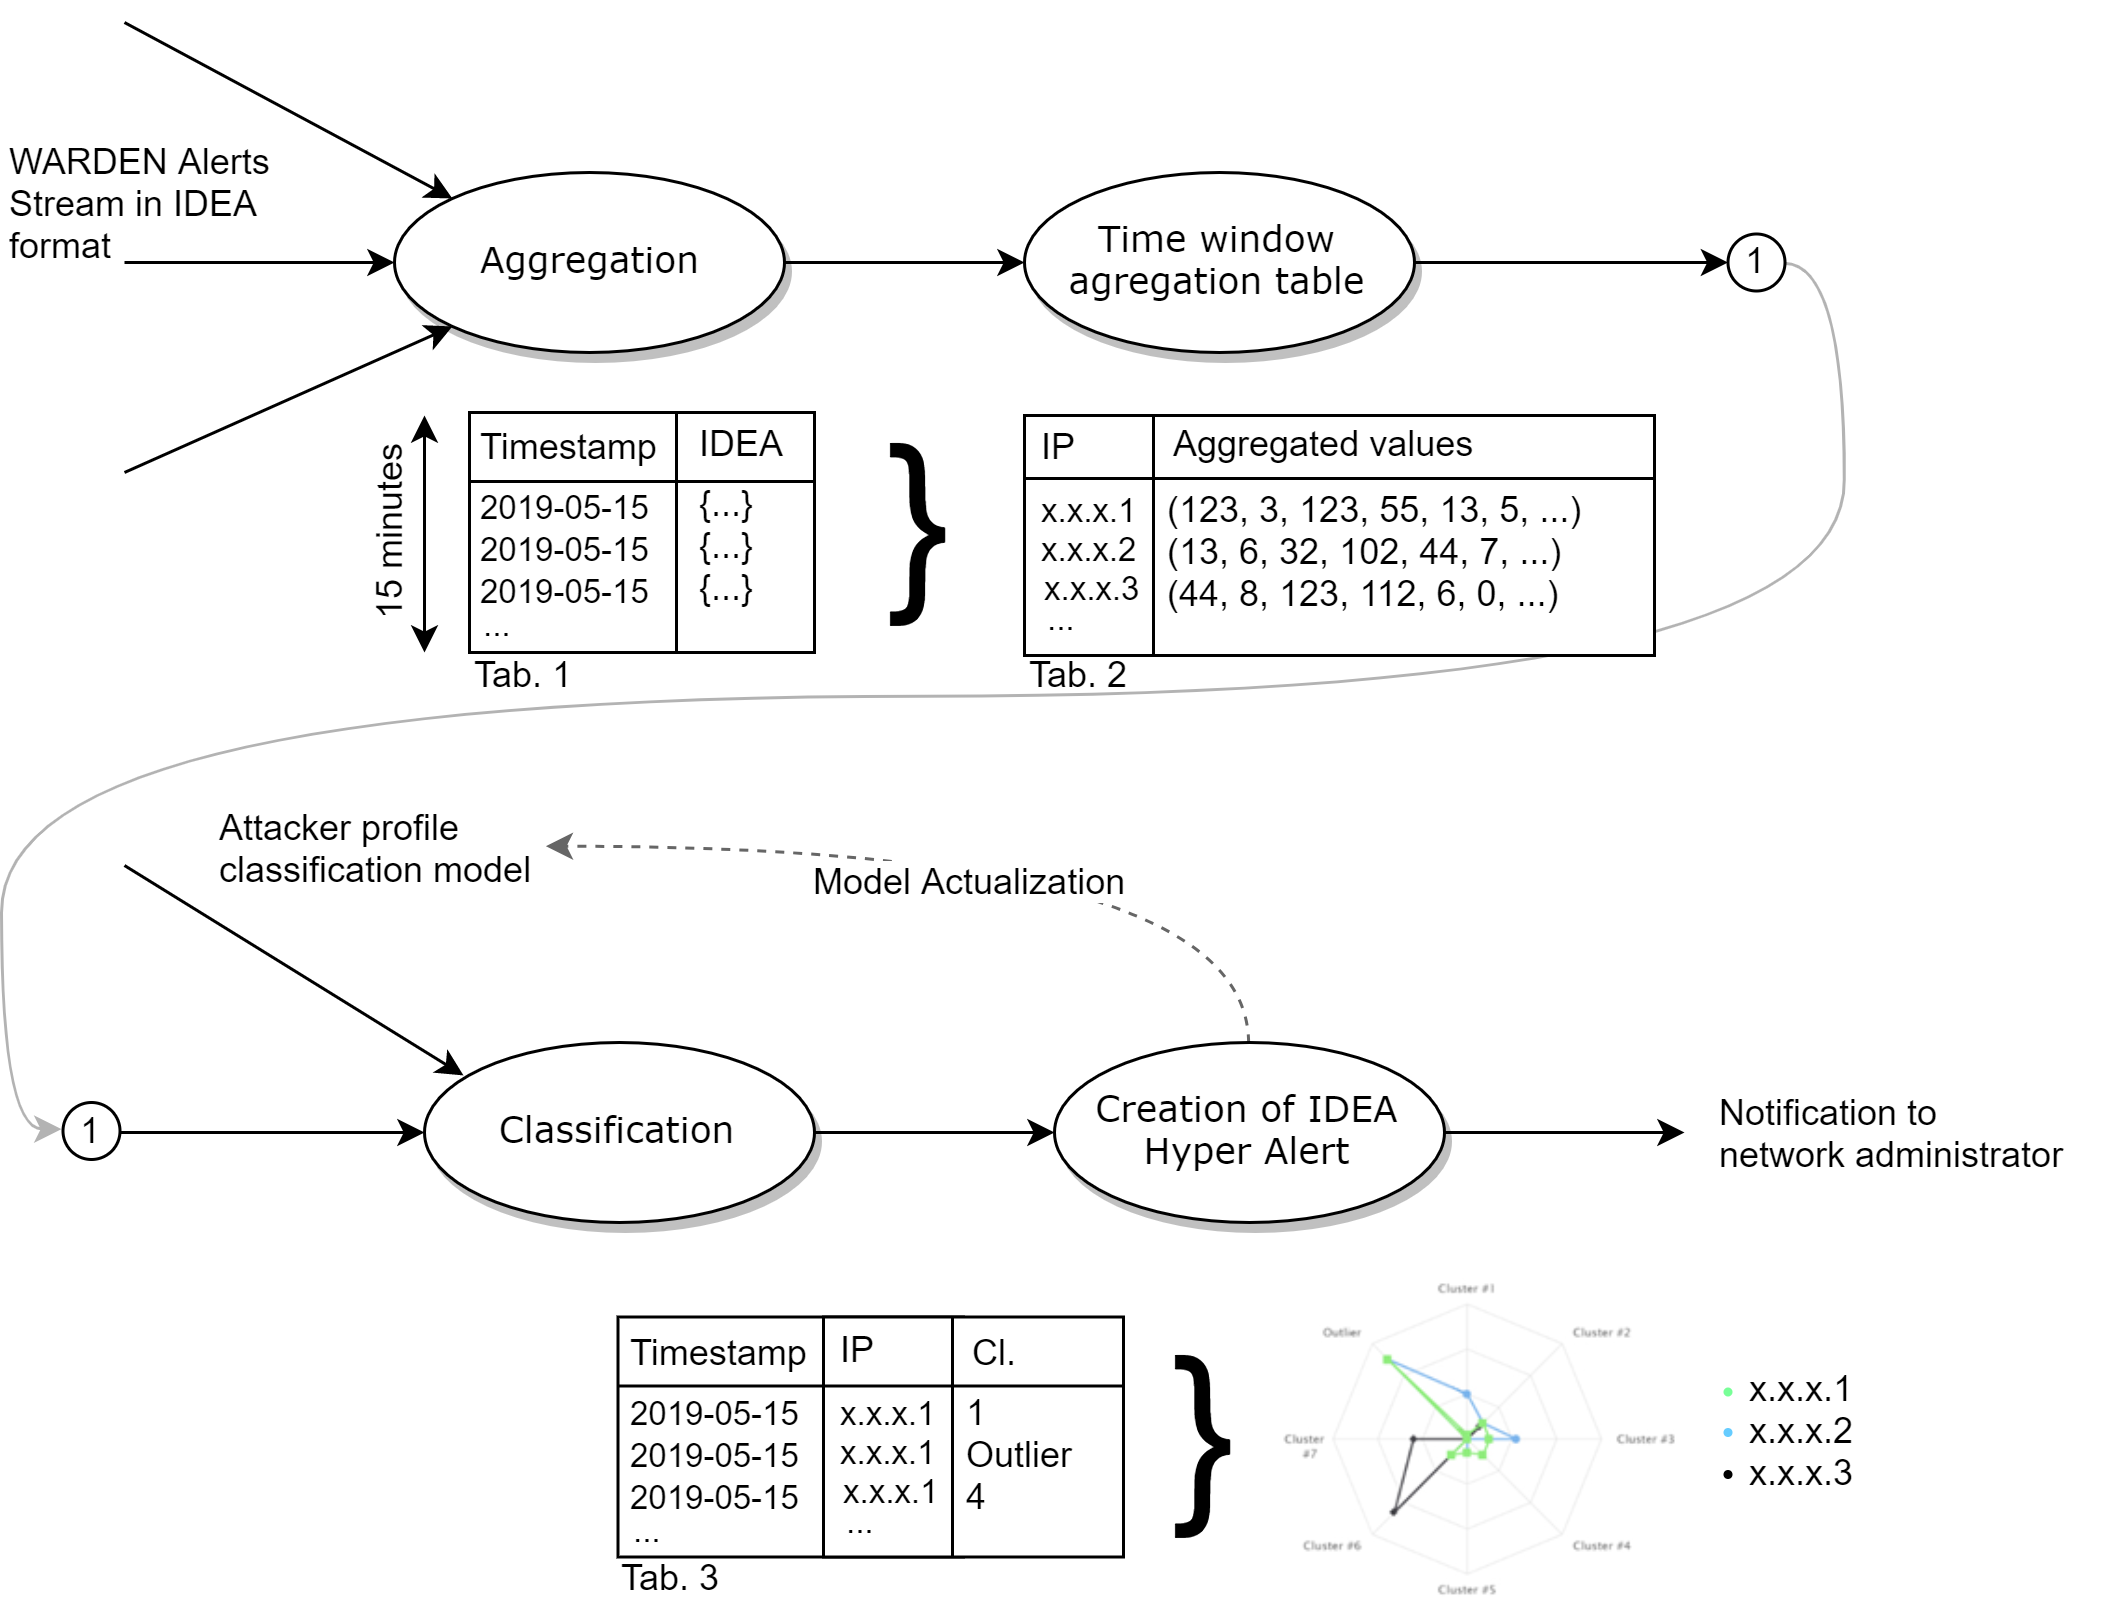
\includegraphics[width=9cm]{images/main-scheme.png}}
\caption{Security data flow stream processing scheme, to network administrator notification.} 
\label{fig1}
\end{figure}

After classification, we obtain a table of attackers assigned to clusters. The data of the different classifications over time are aggregated and visualised in the spider graph shown in Fig.~\ref{fig2} according to the number of classifications to the attacker's profile. In the visualisation, we can observe how the behaviour of the attacker had changed in the monitored time (for example, 30 minutes before the attack was detected). The most prominent figure in the monitored chart is membership in the group of the outliers. The main reason for this high frequency is the early stages of scanning our IP addresses during which we still do not have enough data.

\begin{figure}[htbp]
\centerline{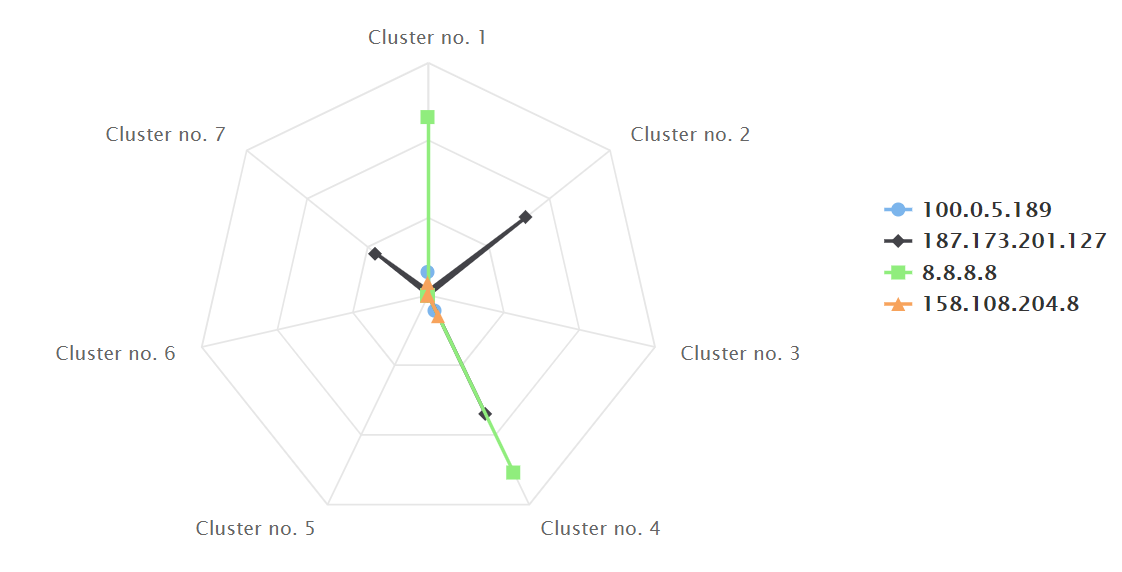
\includegraphics[width=9cm]{images/cluster-ip.png}}
\caption{Visualization of Cluster Allocation by IP Address.}
\label{fig2}
\end{figure}


\subsection{Implementation}
To test our methodology of stream processing cybersecurity data, we have written the application in 
Python version 2.7. We also used the PostgreSQL memory database for storing current window data. Our application has separated each processing steps shown in Fig.~\ref{fig1}. For testing reasons, we do not use streaming input from a real network. Our entire data from 4 weeks was stored in a single table with rows representing single IDEA alert, and every row had a timestamp of receive. Doing it like this, we could process data faster as it would be in production. In our test environment which is Linux kernel 4.19.0-5-amd64 on Intel(R) Xeon(R) E5-2620 v4 @ 2.10GHz with 128GB RAM and SSD drives. We were testing in two separated conditions. First was without dynamic model recalculation, and the second one was recalculating medoid after every classification. We managed to process each 1 minute of latest window IDEA events (it is about 20000 events) to process under 10 seconds for the first condition, and in the second condition, it took 15 - 20 seconds depending on the amount of data in the current window. With this information, we are preparing the environment for production environment for stream processing.

\section{Model for real-time profiling}
In this section, the model for real-time processing of network events and assigning them to a particular profile is described.

\subsection{Aggregation}
The purpose of this module is to receive IDEA alerts and locally create a set of alerts for a specified time. In our experiment, we retained data for the last 15 minutes. An analysis of data collected from the Warden system is difficult without their transformation. For this reason, they had to be preprocessed. Each record from the Warden stands for a security event. In the context of this paper, an attacker, or a threat agent is a specific system entity with a public IP address or several system entities of the same private network subnet using that public IP address to communicate with other devices on the Internet (e.g. using NAT) and perform a threat action. From this data, a table in Fig. \ref{fig1}) with 12 columns were made by transforming data. Each column has its data type. Therefore, it is easier to perform specific operations, for example, numerical operations which were not possible to do directly from the JSON format. Columns in Tab. \ref{tab:ideatrans} represent following properties: (I) ID; (II) source IP address; (III) target IP address; (IV) category; (V) category count; (VI) protocol; (VII) protocol count; (VIII) port; (IX) duration; (X) start timestamp; (XI) end timestamp; and (XII) Internet service provider (ISP). 

However, this table contains attacks, not threat agents; therefore, another transformation was needed. This transformation consists of merging the same source IP addresses, thus creating one entry per one threat agent. 

\begin{table}[ht]
\caption{Transformed IDEA json data to table}
\label{tab:ideatrans}
\centering
\begin{tabular}{|r|l||l|}
\hline
\textbf{Order} & \textbf{Column title} & \textbf{Example value} \\ \hline \hline
1. & ID & 12345 \\ \hline
2. & Source IP & 10.158.x.10 \\ \hline
3. & Target IP & 10.159.x.11 \\ \hline
4. & Category & Recon.Scanning \\ \hline
5. & Category Count & 10 \\ \hline
6. & Protocol & TCP \\ \hline
7. & Protocol Count & 1 \\ \hline
8. & Port & 80 \\ \hline
9. & Duration & 600s \\ \hline
10. & Start Timestamp & 2018-03-18 17:45:15 \\ \hline
11. & End Timestamp & 2018-03-18 17:55:15 \\ \hline
12. & ISP & AS100000 \\ \hline
\end{tabular}
\end{table}

In the final output of this processing step, every threat agent is represented by a 7-dimensional vector. Vectors representing threat agents consist of the following attributes: count of category Recon.Scanning, count of category Availability.DDoS, duration, maximal idleness, minimal idleness, ISP, and count of unique targets. We store the aggregated data in the form of vectors, as shown in Tab. \ref{tab:aggregateddata}. The content that was updated in this table within this processing step will be forwarded to the next processing step for further processing. Processing in this step is described in Algorithm \ref{alg1}. 

\begin{table}[h!]
\caption{Aggregated data table}
\label{tab:aggregateddata}
\centering
\begin{tabular}{|r|l||l|}
\hline
\textbf{Order} & \textbf{Column title} & \textbf{Example value} \\ \hline \hline
1. & Source IP & 10.158.197.10 \\ \hline
2. & Recon.Scanning Count & 156 \\ \hline
3. & Availability.DDoS Count & 155 \\ \hline
4. & Duration & 685s \\ \hline
5. & Maximal Idleness & 80s \\ \hline
6. & Minimal Idleness & 60s \\ \hline
7. & ISP count & 10 \\ \hline
8. & Unique Targets Count & 254 \\ \hline
\end{tabular}
\end{table}

\begin{algorithm}
\caption{Events aggregation and sending to next step}
\label{alg1} % and a label for \ref{} commands later in the document
\begin{lstlisting}
Select 
    IP, 
    Count(CategoryReconScanning),
    Count(CategoryAvailabilityDDoS), 
    Sum(Duration), 
    Max(IdlenessTime), 
    Min(IdlenessTime), 
    ISP, 
    Count(Distinct Targets) 
From TransformedIDEASecurityData 
Group By IP 

# Send Threat Agent Vectors to next step
For (Let Row in Select)  
    Send Row As ThreatAgentVector 
\end{lstlisting}
\end{algorithm}

\subsection{Classification in real-time}
The classification module needs two inputs. The first input is a classification model for profiling attackers. We used a model that was previously calculated from two-week collected security data based on the algorithm from paper \cite{bajtovs2018network}. In this paper we used partitioning around medoids (PAM) clustering method \cite{tuffery2011data} to find representative objects (medoids among the observations of the dataset) of clusters which minimise the sum of the dissimilarities of the observations to their closest representative object. A medoid (centre) is a representative of a cluster, chosen as its most central object. Their model contains the medoids of the seven clusters stored in the vector. This module contains the ranges of attributes in which we can confidently classify future attackers. The second input for this module is the data stream coming from the data preprocessing aggregation. This stream contains IP addresses of their respective vectors of aggregated defined attributes. 

Based on the input data mentioned above, this stream-receiving module classifies the received IP address vector into one of the models defined clusters. If the vector is not included in any of the clusters, then the vector is included in the outlier group. The outlier group represents the attackers whose behaviour is in a completely different way than most attackers. The output of this module is a classified IP address and the creation of a correlated hyperalert enriched with the profile of the attacker where it was included (See Tab. \ref{tab:assignprofile}). Processing in this step is described in Algorithm \ref{alg2}. This code classifies in O(k) where k represents the count of clusters. 

\begin{table}[h!]
    \caption{Correlation of assigned profiles for Source IPs}
    \label{tab:assignprofile}
    \centering
    \begin{tabular}{|l|l|l|}
        \hline
        \textbf{Timestamp} & \textbf{Source IP} & \textbf{Assigned to} \\ \hline \hline
        2018-03-18 17:45:00 & 10.158.197.10 & Cluster 5 \\ \hline
        2018-03-18 17:45:00 & 10.199.197.10 & Outlier \\ \hline
    \end{tabular}
\end{table}

\begin{algorithm}
\caption{Finding minimal vector distance to cluster model center}
\label{alg2}
\begin{lstlisting}
Receive ThreatAgentVector 
Load ClusteringModels 
# |ClusteringModels| = 7

Let MinDistance = Infinity 
Let MinVector = Outlier 
For(Let ClusterName, ClusterVector In ClusteringModels) 
    Set Distance = FindDistanceBetweenVectors(ClusterVector, ThreatAgentVector) 
    If(Distance != null OR Distance < MinDistance) 
        MinDistance = Distance 
        MinVector = ClusterName 
Send MinVector As ThreatAgentClusterName 
Send ThreatAgentVector As ThreatAgentVector 
\end{lstlisting}
\end{algorithm}


\subsection{Classification model actualization}
The current processing solution proposed so far has one disadvantage. In the beginning, the calculated model from the previous paper was calculated on a two-week data sample, and it is recommended to update clustering at regular intervals to keep the application up to date. However, such a recalculation has nothing to do with stream processing, and it would be an external input to the proposed solution for us. That is the reason why we have also focused on dynamic model updates. We have modified the algorithm so that after successful classification of a new record it could update the centre of the cluster to which it was assigned. We have used the weighted average to recalculate the centre of the cluster. The model automatically updated for two weeks was compared to a statically calculated model according to \cite{bajtovs2018network}. An important observation was that the dynamic update did not work towards the same model. The main reason why the models were different over the same period and the same security data is the following: in stream processing, model updates on partially received aggregated records. That is the reason why one threat agent can update the cluster model multiple times to the end of his activity. Processing in this step is described in Algorithm \ref{alg3}.

\begin{algorithm}
\caption{Finding minimal vector distance to cluster model center}
\label{alg3}
\begin{lstlisting}
Receive ThreatAgentVector 
Receive ThreatAgentClusterName 
Load ClusteringModels 

If(ThreatAgentVector != Outlier)  
    Let ThreatAgentClusterVector = ClusteringModel.Get(ThreatAgentClusterName) 
    NewThreatAgentClusterVector = ThreatAgentClusterVector.RecalcWithWeightAverage(ThreatAgentVector) 
    ClusteringModels.Change(ThreatAgentClusterName, NewThreatAgentClusterVector)
    Save ClusteringModels 
\end{lstlisting}
\end{algorithm}

After running the number of PAM iterations on different data, we figured out that it is needed to name each calculated cluster. The main problem began when the clustering model was recalculated, and the number of clusters was exchanged between them. We added an algorithm which classified each cluster from a new model. Then this algorithm assigned the same numbers to closest clusters. This cluster ordering helped us to stabilise clusters and made them more precise in time.

\subsection{Results}
Within this chapter, we have focused more closely on the analysis of cluster development over four weeks. In Fig.~\ref{fig3}, we can see input data for creating threat agent models. The total number of events (green) and the total number of attacks (yellow) can give us a general picture of the overall state of security events in our dataset.

\begin{figure}[htbp]
\centerline{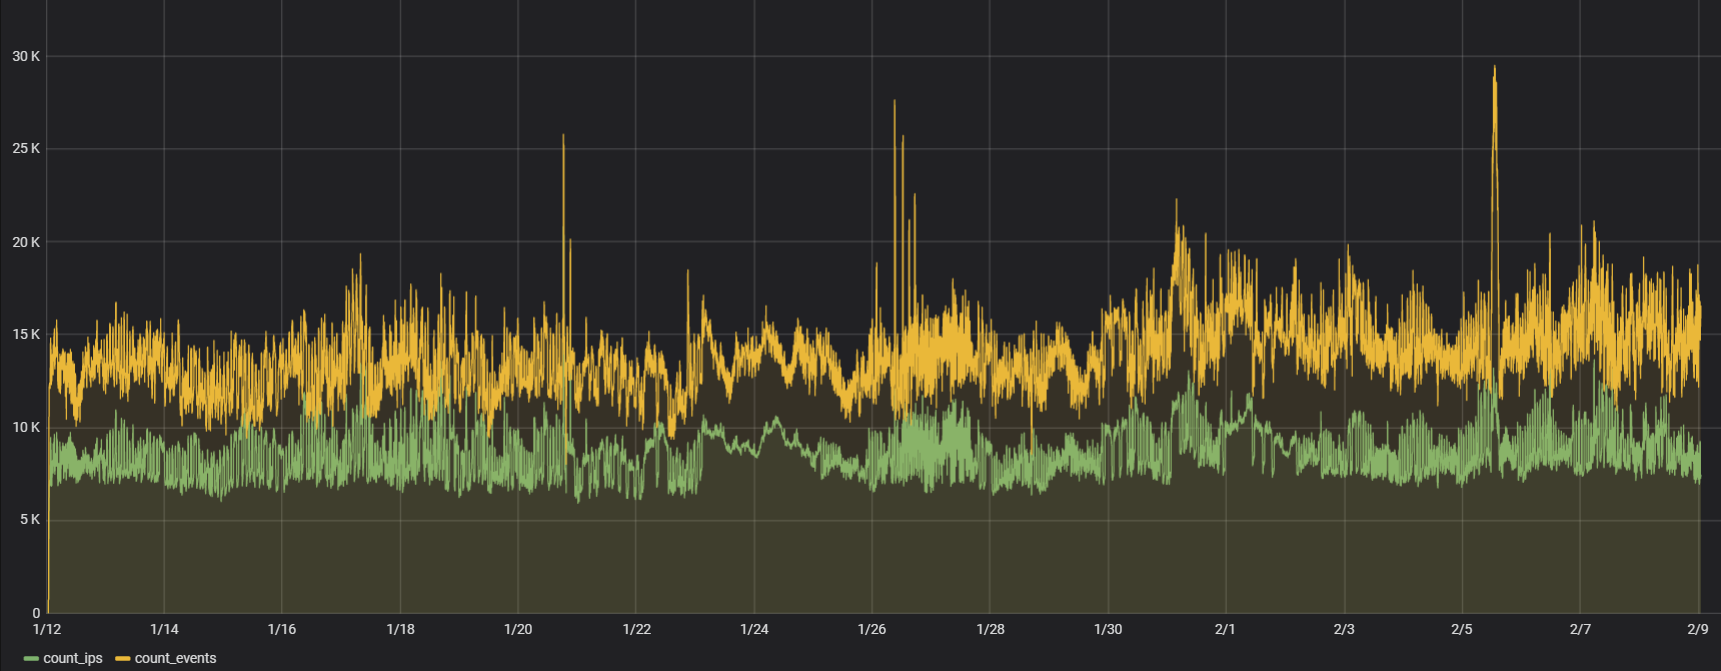
\includegraphics[width=9cm]{images/fig3.png}}
\caption{Total number of security events (yellow) and IP addresses (green) over a period of 4 weeks.} 
\label{fig3}
\end{figure}

Following figures \ref{fig4} and \ref{fig5} represents distribution of unique IP addresses in time window to the clusters. In Fig.~\ref{fig4} we can see that each cluster oscillates around a specific value, but several local maxima can be observed. These are not caused by a higher number of IP addresses, but by a change in the distribution of individual threat agent profiles.

\begin{figure}[htbp]
\centerline{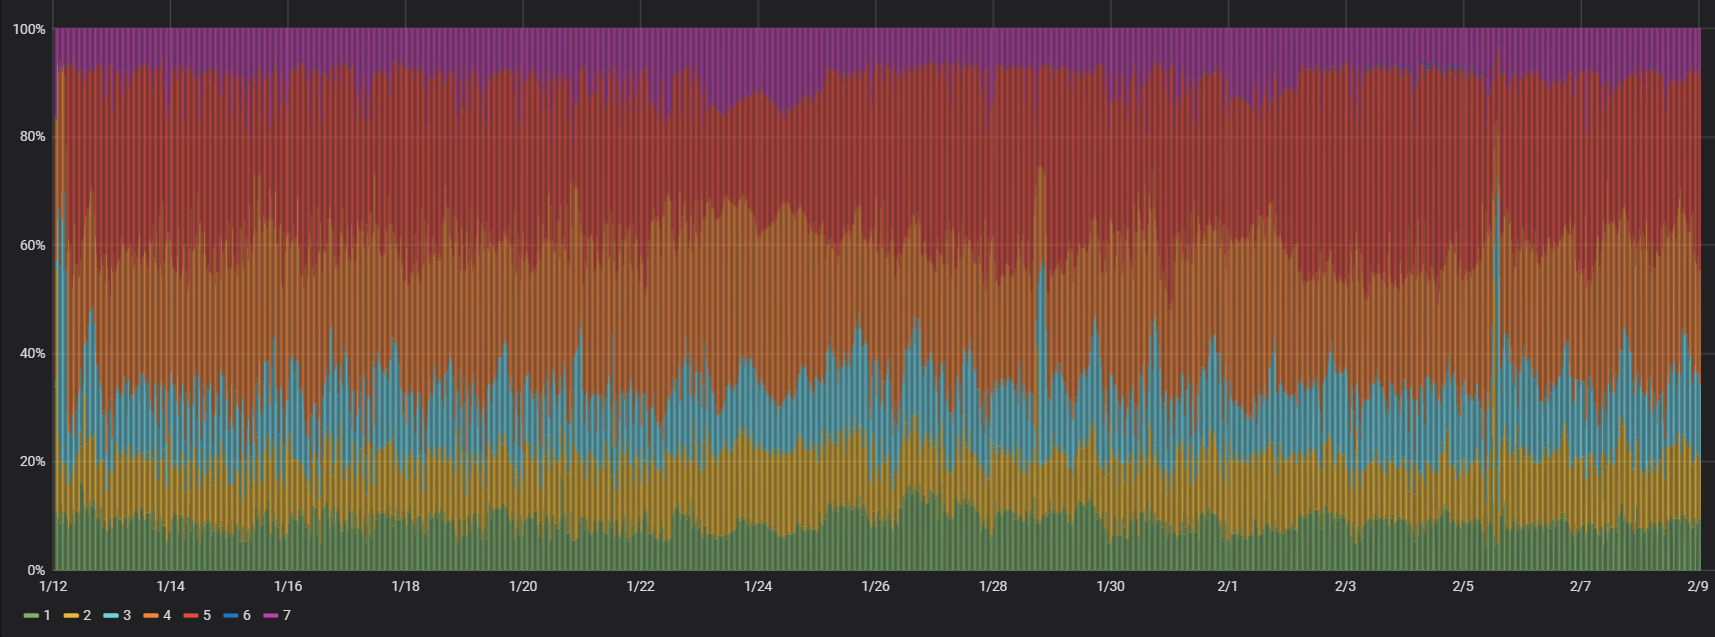
\includegraphics[width=9cm]{images/fig4.png}}
\caption{Percentage distribution of clusters over a period of 4 weeks.} 
\label{fig4}
\end{figure}

The percentage distribution of the individual profiles within four weeks is shown in Fig.~\ref{fig4}. The most significant changes can be seen in cluster no. 3 (turquoise). Following figure Fig.~\ref{fig5} is zoomed into date of January 28, 2018, from 6:30 pm to 9:40 pm. The threat agent is characterised by, on average, seven different attack targets with a low span between individual security incidents.

\begin{figure}[htbp]
\centerline{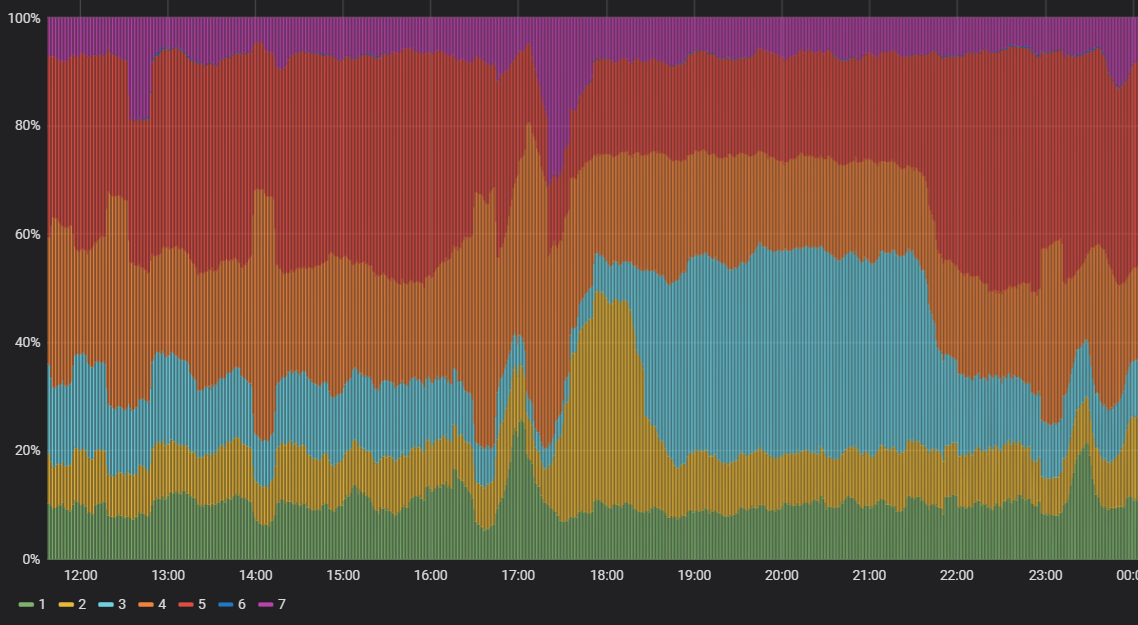
\includegraphics[width=9cm]{images/fig5.png}}
\caption{Percentage distribution of clusters on 28.1.2019 from 12:00 to 24:00} 
\label{fig5}
\end{figure}


\section{Conclusion and future works}
In this paper, we discussed streaming applications to detect attackers in a computer network. We use security data from the Warden system as input security data. We have proposed a procedure for aggregation and classification these data by stream processing. Since only the changed data is transferred from one step to another in the streaming process, we can minimise the complexity of the calculations. We can also see that the modules are relatively simple for processor power. This results in a significant reduction in detection from the original two-week reports for immediate attacker profiling, as well as alerts to network administrators at the first hints of an attack in or towards their computer network. This is a big difference comparing to previous research.

Other questions that have arisen in the design of this solution include the analysis of how large of a time window can be used (currently 15 minutes). Another question for future research is the ability to reduce the weight of older activity to increase the time window to one hour. It is also advisable to check whether setting the minimum values (threshold) in each aggregated attribute helps reduce false positives when creating hyper alerts at the time of classification. Also, the opened question is whether vectors that do not pass the filter can affect the dynamic modification of the model. Smooth transition of the attackers between the profiles raised the question of whether we can evaluate the strength in individual profiles.

\section*{Acknowledgment}
This research is funded by project No. VVGS-PF-2019-1062, project No. VEGA/A-1/0056/18, and Slovak Research and development agency (APVV) project under contract No. APVV-17-0561.

%\section*{References}
\bibliographystyle{./bibliography/IEEEtran}
\bibliography{./bibliography/IEEEbib.bib}

\end{document}
